\documentclass[10pt,journal]{IEEEtran}
\IEEEoverridecommandlockouts
\usepackage[spanish,es-tabla]{babel}
\renewcommand{\baselinestretch}{1.5}     %interlineado
\usepackage[utf8]{inputenc} 
\usepackage[square,numbers]{natbib}
\bibliographystyle{abbrvnat}
\usepackage{float}                      % para usar [H]
\usepackage[table,xcdraw]{xcolor}
\usepackage{amsmath,amssymb,amsfonts}
\usepackage{graphicx}
\usepackage{textcomp}
\usepackage{xcolor}

\def\BibTeX{{\rm B\kern-.05em{\sc i\kern-.025em b}\kern-.08em
    T\kern-.1667em\lower.7ex\hbox{E}\kern-.125emX}}

%---------------------------------------------------
\begin{document}

\title{Dispositivos de Almacenamiento Actuales\\}
%--------------------------------------------
\author{\IEEEauthorblockN{Ciara Mendez Cruz}
\IEEEauthorblockA{\textit{} \\
\textit{Universidad Nacional de Trujillo} \\ 
\textit{Trujillo, Perú} \\
t022700920@unitru.edu.pe}}
\maketitle
%-------------------------------------------
\begin{abstract}
Los dispositivos de almacenamiento actuales se emplean para almacenar toda la información del ordenador tales como el sistema operativo, nuestros archivos, programas, etc. Entre ellos tenemos al disco duro, el disco duro SSD, CD-ROM. Debido a que cada día se multiplica la cantidad de datos almacenados casi de forma exponencial, se han creado formas de poder guardar y usarlos por un largo tiempo, es así que, gracias a Softwares tales como: SAS y el Software PolyAnalyst especializados en minería de datos, brindan la solución a ello y permiten trabajar con volúmenes de datos inmensos, asimismo ocurre con el almacenamiento en la nube como: Amazon, IBM y Google, que facilitan a los usuarios almacenar sus datos sin tener ningún dispositivo físico. 
\end{abstract}

\begin{IEEEkeywords}
almacenamiento, tecnologías, datos, dispositivos, software.
\end{IEEEkeywords}

\section{\textbf{Introducción}}
Los dispositivos de almacenamiento son indispensables para el uso del ordenador, pues en ellos está grabado e instalado toda la información que necesitamos y poseemos. Desde que se creó la primera unidad de almacenamiento hasta ahora, éstas han evolucionado enormemente, las primeras unidades de almacenamiento han quedado obsoletas para lo que se requiere en estos días. Por ello, en este informe se presenta información respecto a los dispositivos de almacenamiento actuales, el cual está organizado de la siguiente manera: en primer lugar, se explican los conceptos teóricos de los dispositivos de almacenamiento, luego se da énfasis en los sistemas de almacenamiento de datos digitales actuales, los cuales están presentes en la minería de datos y en las tecnologías que almacenan grandes volúmenes de datos.
%------------------------------------------
\section{\textbf{Dispositivos de almacenamiento}}
\vspace{-22 mm}
\subsection{\textbf{Conceptos teóricos}}
\vspace{-14 mm}
Los dispositivos de almacenamiento son elementos de hardware que se emplean para almacenar toda la información del ordenador tales como el sistema operativo, nuestros archivos, programas, etc.\par La importancia de ellos en nuestros equipos es vital pues en ellos está instalado o grabado todo aquello que requiramos para poder hacer usar de estos.
Actualmente se utilizan tres tecnologías diferentes para construir nuestros dispositivos de almacenamiento y son los siguientes:\par

\subsubsection{\textbf{Dispositivos de almacenamiento magnéticos}}\par
Estos dispositivos se caracterizan porque usan propiedades magnética de ciertos materiales para almacenar información. 
Un claro ejemplo de este tipo de dispositivo de almacenamiento son los Discos Duros.
\begin{itemize}
    
    \item \textbf{Discos duros:} \par
    Los discos duros (HDD, Hard Disk Drive) constituyen el medio de almacenamiento de información más importante del ordenador. Permiten almacenar y recuperar gran cantidad de información.
    Un disco duro es una caja herméticamente cerrada, en cuyo interior se encuentra un conjunto de componentes electrónicos y mecánicos capaz de sincronizar los dos motores y las acciones de las cabezas de lectura/escritura.\citep{montaje}
\begin{figure}[H]
 \begin{center}
       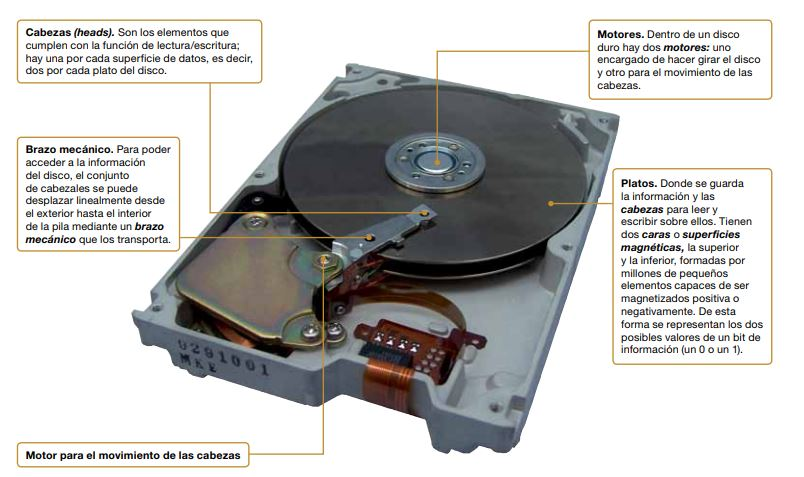
\includegraphics[width=8.5cm, height=5cm]{figuras/1.JPG}
      \caption{Componentes de una unidad de disco duro.}
      \label{f1} 
      \end{center}
\end{figure}
De la Figura~\ref{f1} se puede observar que el disco es en realidad una pila de discos llamados platos que almacenan la información magnéticamente. Los diferentes platos que forman el disco giran a una velocidad constante y no cesan mientras el ordenador está encendido. Cada cara del plato tiene asignado uno de los cabezales de lectura/escritura.
\end{itemize}
%---------------------------------------------------------------------------
\subsubsection{\textbf{Dispositivos de almacenamiento en estado sólido (en inglés SSD)}}Estos dispositivos se caracterizan porque usan transistores especialmente diseñados para almacenar una pequeña carga eléctrica. De esta forma, adquieren dos estados, el estado en el que poseen una carga eléctrica y el estado en que no la poseen. El dispositivo es capaz de reconocer esos estados e interpretarlos como los dos estados del binario (1 y 0). Un claro ejemplo de este tipo de dispositivo de almacenamiento son los Discos Duros SSD.\citep{montaje}
%\vspace{-1.5mm}
\begin{itemize}
    \item \textbf{Discos duros SSD:}\par
    Los discos duros SSD (Solid-State Drive) basan sus memorias en no volátiles (como las memorias flash) o volátiles como la SDRAM, en lugar de estar basados en tecnologías móviles como los discos de platos tradicionales. Al no tener elementos móviles, son mucho más rápidos y silenciosos, no desprenden calor, resisten mucho mejor los golpes y su consumo energético es inferior. Pueden suponer una revolución en los ordenadores portátiles, ya que multiplican la duración de la batería y son más seguros.
%-------------------------------------   
\begin{figure}[H]
 \begin{center}
       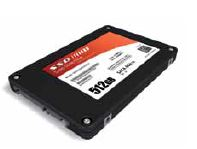
\includegraphics[width=4cm, height=3cm]{figuras/2.JPG}
      \caption{Disco SSD con memoria no volátil (memoria flash).}
      \label{f2} 
      \end{center}
\end{figure}
%-------------------------------------
\begin{table}[H]
\centering
\caption{Ventajas e inconvenientes de los discos SSD.}
\label{tab1}
\begin{tabular}{cl}
\rowcolor[HTML]{329A9D} 
\multicolumn{2}{c}{\cellcolor[HTML]{329A9D}{\color[HTML]{000000} \textbf{Unidades SSD frente a los Discos Duros}}} \\ \hline
\rowcolor[HTML]{9B9B9B} 
\multicolumn{1}{|c|}{\cellcolor[HTML]{9B9B9B}{\color[HTML]{000000} \textbf{Ventajas}}} & \multicolumn{1}{c|}{\cellcolor[HTML]{9B9B9B}{\color[HTML]{000000} \textbf{Inconvenientes}}} \\ \hline
\multicolumn{1}{|l|}{{\color[HTML]{000000} \begin{tabular}[c]{@{}l@{}}Consumen menos energía.\\ Pueden llegar a tener más\\ velocidad.\\ Menor peso, tamaño y ruido.\\ El arranque es más rápido.\\ Con el tiempo, pueden llegar a\\ tener mayor capacidad.\\ Puede sobrevivir a una caída.\end{tabular}}} & \multicolumn{1}{l|}{{\color[HTML]{000000} \begin{tabular}[c]{@{}l@{}}Actualmente los precios\\ son más altos.\\ Periodo de vida más limitado.\\ Menor velocidad en\\ operaciones de I/O\\ secuenciales.\\ Menor recuperación en\\ caso de fallo mecánico.\\ No hay un estándar de\\ velocidad.\end{tabular}}} \\ \hline
\end{tabular}
\end{table}
%-------------------------------------
\end{itemize}
%-------------------------------------
\subsubsection{\textbf{Dispositivos de almacenamiento ópticos}} Estos dispositivos se caracterizan porque basan su tecnología en leer con un láser una superficie reflectante. En la misma existen unas pistas que pueden o no tener pequeñas perforaciones. El dispositivo lector emite un rayo láser, que incide en la pista y se reflecta (“rebota”) en la misma. Dicho dispositivo posee un receptor al que llega el láser cuando “rebota” contra la pista cuando no tiene una perforación. Si el láser incide en una perforación no es reflectado al receptor.\citep{montaje}
Un claro ejemplo de este tipo de dispositivo de almacenamiento son los CD-ROM.

\begin{itemize}
    \item \textbf{CD-ROM:} \par
    El CD (Figura ~\ref{f3}) apareció por primera vez en 1982 en formato de audio. Los CD-ROM aparecieron en 1984; eran muy caros, por lo que hubo de pasar un tiempo para que reemplazaran a los disquetes como medio de distribución de software. Estos permitían almacenar hasta 700 MB. Actualmente numerosos productos de software necesitan varios CD-ROM.
%----------------------------------    
\begin{figure}[H]
 \begin{center}
       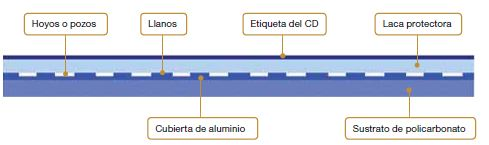
\includegraphics[width=8cm, height=3cm]{figuras/3.JPG}
      \caption{Capas de un CD.}
      \label{f3} 
      \end{center}
\end{figure}
\end{itemize}
%----------------------------------    
\section{\textbf{Sistemas de almacenamiento de datos digitales actuales}}
\subsection{\textbf{Minería de Datos}}
En la actual sociedad de la información, donde cada día se multiplica la cantidad de datos almacenados casi de forma exponencial, la minería de datos es una herramienta fundamental para analizarlos, explotarlos y sobre todo almacenarlos de forma eficaz para los objetivos de cualquier organización.\par
La definición de Minería de Datos puede variar entre los diferentes investigadores ya sean estadísticos, analistas de datos u otros. A continuación se muestran algunas definiciones:
\begin{itemize}
    \item "La minería de datos puede definirse como el proceso de extraer conocimiento útil y comprensible, previamente desconocido, a partir de grandes volúmenes de datos” \citep{gonzalez}
    \item "La minería de datos es el análisis de habitualmente grandes, series de datos para encontrar relaciones inesperadas y resumir la información de nuevas maneras que sean entendibles y útiles por el propietario de los datos” \citep{1999}
\end{itemize}
\par Ambos autores \citep{gonzalez} y \citep{1999}, coinciden en que la minería de datos es trabajar con grandes cantidades de datos. 
Por lo que se podría decir que este proceso en la actualidad es la nueva forma de almacenar información, sin requerir dispositivos físicos, sino más bien solamente digitales, específicamente softwares.\par
Muchas organizaciones emplean la minería de datos para el almacenamiento y análisis de su información, algunos ejemplos de softwares son los siguientes:
\begin{itemize}
    \item \textbf{SAS Enterprise Miner:} \par
    Su compañía es SAS (Figura ~\ref{f4}), es una solución de minería de datos que permite incorporar patrones inteligentes a los procesos de marketing, tanto operativos como estratégicos. 
    \begin{figure}[H]
        \begin{center}
            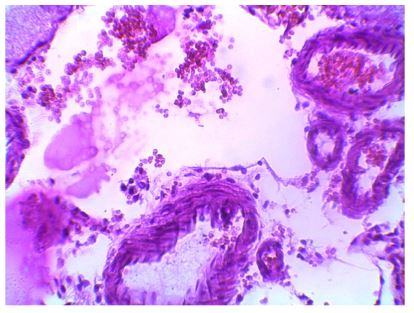
\includegraphics[width=4cm, height=2cm]{figuras/4.PNG}
            \caption{Logotipo de SAS.}
            \label{f4} 
         \end{center}
    \end{figure}
    \par El software de SAS (Figura ~\ref{f5}), es un sistema de entrega de información que provee acceso transparente a cualquier fuente de datos, incluyendo archivos planos, archivos jerárquicos, y los más importantes manejadores de bases de datos relacionales.\par También incluye su propia base de datos de información para almacenar y manejar los datos, es decir, un "data warehouse". También soporta los principales protocolos de comunicación, cubre los cinco modelos de procesamiento cliente/ servidor de acuerdo a Gartner Group y cumple con las 12 reglas de OLAP. \par El sistema soporta un amplio rango de aplicaciones, destacándose el análisis estadístico, análisis gráfico de datos, análisis de datos guiado, mejoramiento de la calidad, diseño experimental, administración de proyectos, programación lineal y no lineal, generación de reportes y gráficas, manipulación y despliegue de imágenes, sistemas de información geográfica, visualización multidimensional de datos, aplicaciones de multimedia, así como los sistemas de información ejecutiva.
%----------------------------------       
\begin{figure}[H]
 \begin{center}
       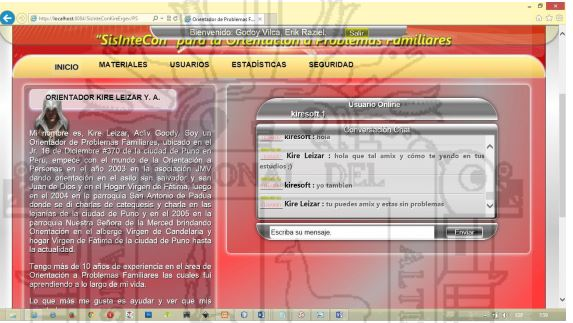
\includegraphics[width=8cm, height=5cm]{figuras/5.JPG}
      \caption{Software SAS.}
      \label{f5} 
      \end{center}
\end{figure}
\end{itemize}
%----------------------------------
\vspace{5 mm}
\begin{itemize}
    \item \textbf{PolyAnalyst de Megaputer:}\par
    Es un sistema de minería de datos premiados de la multiestrategia para descubrir la forma exacta de relaciones funcionales ocultadas en datos. Además de descubrir reglas y algoritmos, PolyAnalyst les presenta explícitamente en el una forma simple y fácil de entender. En la fundación de PolyAnalyst (Figura ~\ref{f6}) tiene un lenguaje de programación interno universal capaz de expresar reglas y algoritmos arbitrarios.\par
\begin{figure}[H]
 \begin{center}
       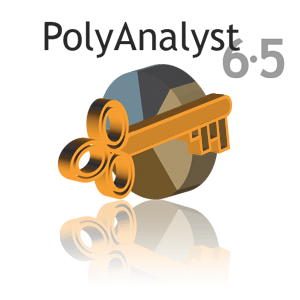
\includegraphics[width=8cm, height=4cm]{figuras/7.PNG}
      \caption{Logotipo de PolyAnalyst.}
      \label{f6} 
      \end{center}
\end{figure}
    Su compañía es Megaputer líder en negocios y software inteligentes para web. Ofrece las mejores herramientas para data mining, text mining y web mining.(Figura ~\ref{f7}) 
\begin{figure}[H]
 \begin{center}
       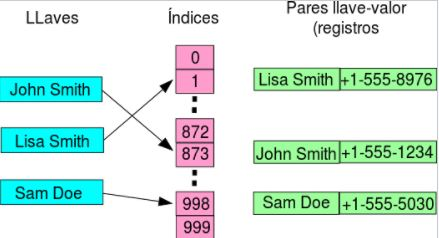
\includegraphics[width=6cm, height=4cm]{figuras/6.PNG}
      \caption{Software PolyAnalyst.}
      \label{f7} 
      \end{center}
\end{figure}    
\end{itemize}
Entonces, ¿Por qué usar Minería de Datos?, porque permite a las empresas, ALMACENAR, explorar y comprender los datos e identificar patrones, relaciones y dependencias que impactan en los resultados finales.\par Además, ahorra grandes cantidades de dinero a una empresa y abre nuevas oportunidades de negocios asimismo contribuye a la toma de decisiones tácticas y estratégicas.(Figura ~\ref{f8})
\begin{figure}[H]
 \begin{center}
       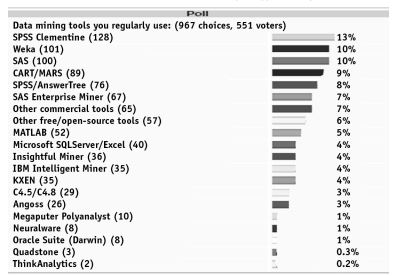
\includegraphics[width=8cm, height=4cm]{figuras/8.JPG}
      \caption{Herramientas de Minería de Datos usadas habitualmente.\citep{Poll}}
      \label{f8} 
      \end{center}
\end{figure}
%-----------------------------------------
\subsection{\textbf{Tecnologías para el almacenamiento de grandes volúmenes}} El desarrollo de la tecnología en almacenamiento sigue presentando nuevas formas como la Memoria de Cambio de Fase (PCM: Phase Change Memory), que de acuerdo con \citep{gopala}, tiene la bondad de facilidad de integración, escalabilidad, velocidad y resistencia; esta podría ser una opción en un sistema de almacenamiento de grandes capacidades de datos.
\par Además, sus bondades prometen ser memorias no volátiles de próxima generación \citep{yoon2013integrated}, considerando que muchas aplicaciones modernas exigen cada vez más para el manejo de grandes cantidades de datos. \par Nos encontramos ante una etapa de transición, de modo que las unidades de disco duro tradicional, sólido y memorias de PCM en este tiempo nos ayudarán a resolver nuestros problemas de almacenamiento de grandes datos.\par Este desarrollo tecnológico ha permitido que los centros de datos dedicados al almacenamiento estén estructurados de una o varias combinaciones de las siguientes cuatro formas: DAS, SAN, NAS y almacenamiento en la nube. A continuación, se describe cada uno de ellos:
%----------------------------------    
\begin{enumerate}[1.]
    \item \textbf{DAS (Direct Attached Storageo):} \par
    DAS es una de las formas más sencillas y tradicionales del almacenamiento de conexión directa, donde las unidades de disco se encuentran conectadas directamente con los servidores o hosta través de una interfaz de datos SCSI o IDE (Figura ~\ref{f9}). \par Las conexiones en DAS tienen muchas ventajas, tales como: su instalación es fácil; el software es poco complejo; el costo en mantenimiento es bajo; la tecnología presenta madurez técnica, buena compatibilidad y, relativamente, es de menor gasto. Sin embrago, su deficiencia aparece en cuatro aspectos: (1) la capacidad de almacenamiento está limitada por el servidor; (2) su rendimiento de almacenamiento es directamente afectado por el servidor; (3) los servidores dispersos geográficamente se limitan al intercambio de información y gestión cuando se tiene un servidor aislado; (4) la carga de almacenamiento de datos y el acceso en el servidor hará en general tener un pobre rendimiento.
    \begin{figure}[H]
        \begin{center}
            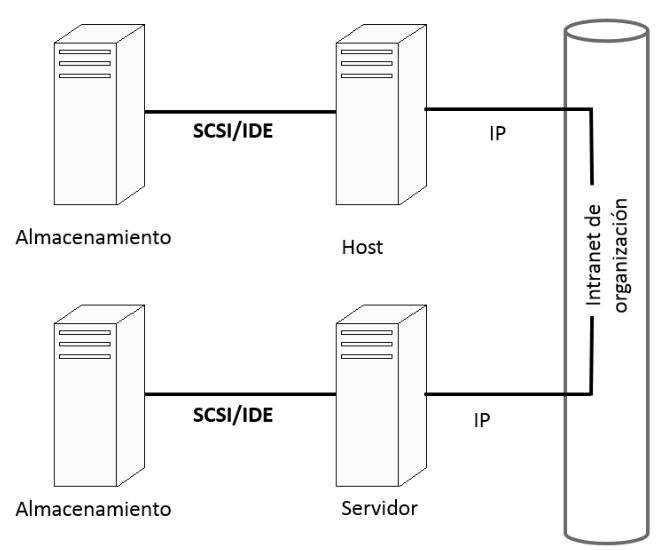
\includegraphics[width=5cm, height=3cm]{figuras/DAS.JPG}
             \caption{Almacenamiento de Conexión Directa (DAS).\citep{vazquez}}
             \label{f9} 
        \end{center}
    \end{figure}
    \item \textbf{NAS (Network Attached Storage):} \par
    El Almacenamiento Conectado en Red o NAS es un dispositivo que se conecta a la red y provee un almacén de datos que permite a varios hosts acceder al mismo lugar de almacenamiento a través de una red IP.\par El espacio de almacenamiento se presenta en la red con un nodo dedicado a través de un servidor de archivos, aunque en sistemas recientes este dispositivo puede ser un dispositivo inmerso en la red (Figura ~\ref{f10} ).\par NAS y LAN están en la misma red física; por lo tanto, NAS depende de ciertas características de LAN. Para ello necesita un gran ancho de banda en red y de muy alta potencia de procesamiento del CPU: cuando no se cumplen estas condiciones, la red se congestiona y su rendimiento se reduce.
    \begin{figure}[H]
        \begin{center}
            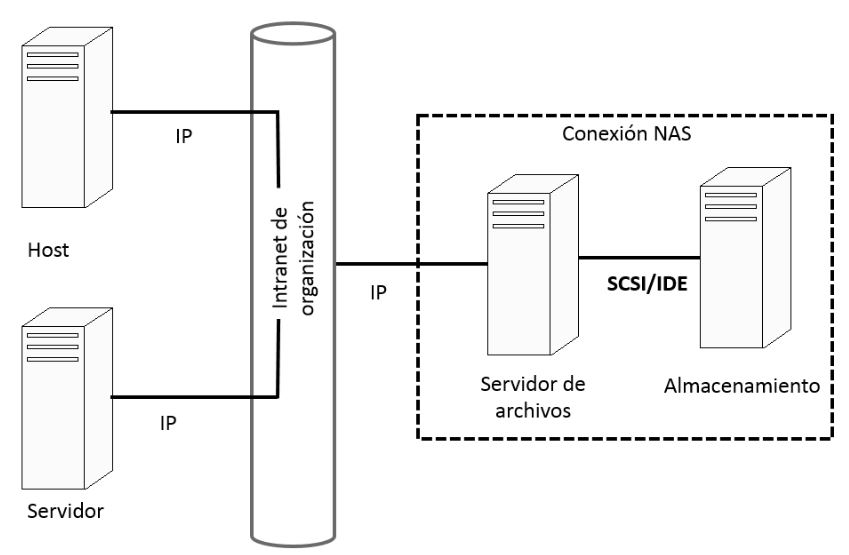
\includegraphics[width=5cm, height=3cm]{figuras/NAS.JPG}
            \caption{Almacenamiento Conectado en Red (NAS).\citep{vazquez}}
            \label{f10} 
      \end{center}
    \end{figure}
    \item \textbf{SAN (Storage Area Network):} \par
    SAN se centra en el almacenamiento de datos utilizando una topología de red flexible, además, con conexiones de fibra óptica que permiten alta velocidad en la transferencia de datos; ofrece la conmutación entre múltiples nodos (Figura ~\ref{f11}). \par Sin duda, SAN es otro enfoque de almacenamiento compartido que a menudo se usa en la nube. En SAN,la gestión del almacenamiento de datos se encuentra relativamente independiente a la red de área local, con el fin de lograr el máximo grado de intercambio de datos, así como la extensión del sistema \citep{sadlier}.
    \begin{figure}[H]
        \begin{center}
            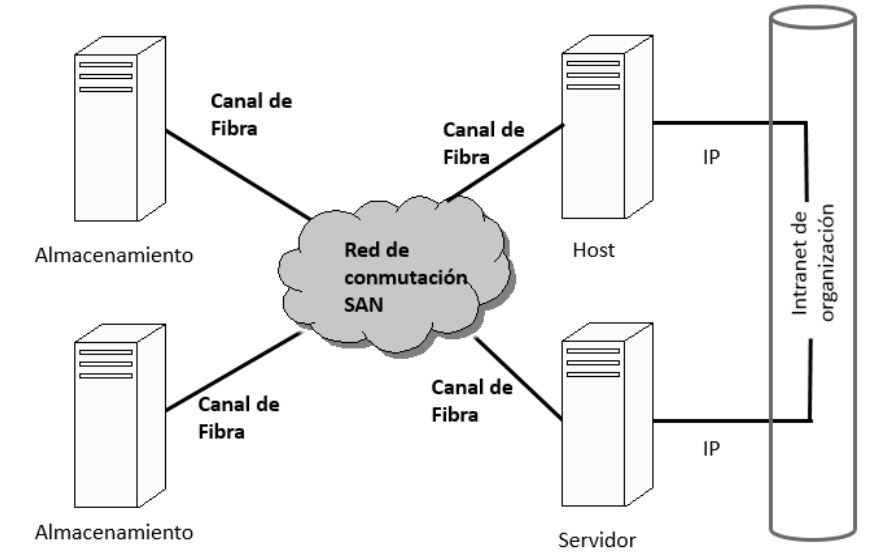
\includegraphics[width=5cm, height=3cm]{figuras/SAN.JPG}
            \caption{Red de Área de almacenamiento (SAN).\citep{vazquez}}
            \label{f11} 
      \end{center}
    \end{figure}
    \item \textbf{Almacenamiento en la nube:} \par
    El desarrollo del almacenamiento de datos en la nube, mejor conocido como cloud computing, se da gracias al uso de equipos virtuales \citep{fur}; implica una infraestructura informática invisible para el usuario, pero al utilizarla parece que se tuviera un equipo físico real, permitiendo la gran ventaja de determinar el número de procesamiento, el sistema operativo, el tamaño de memoria RAM y de disco de almacenamiento. \par El nombre de cloud computing proviene de la utilización del símbolo con forma de nube o cloud, que es el diagrama usado en sistemas como una abstracción para determinar internet, mientras que computing implica la informática.\par
    \begin{itemize}
        \item \textbf{Proveedores de servicios de almacenamiento en la nube:}\par
            \begin{enumerate}[]
                \item \textbf{Amazon:} \par
            Es un sitio web de comercio electrónico; no solo es la librería virtual más grande del mundo, sino que es una de los principales proveedores de servicios en la nube y, además de su eficiencia, presenta mejor garantía de servicio.\par El servicio de Amazon Simple Storage Service es una interfaz de servicios web que puede utilizarse para almacenar y recuperar grandes cantidades de datos, en cualquier momento y desde cualquier parte de la web.\par Es una infraestructura de almacenamiento de datos altamente escalable, fiable y de rápida transferencia.
            \begin{figure}[H]
                \begin{center}
                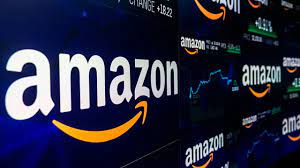
\includegraphics[width=5cm, height=3cm]{figuras/amazon.jpg}
                \caption{Amazon.}
                \label{f12} 
                \end{center}
            \end{figure}
            \item\textbf{IBM:} \par
            Los servicios de cloud computing de IBM incluyen también el almacenamiento con IBM Smart Business Storage Cloud, el cual surgió por el crecimiento en los volúmenes de datos y la diversidad de formatos de archivo. \par Así esta solución permite que los usuarios tengan un acceso eficiente, rentable y experimenten una disminución del rendimiento e interrupciones. En este sentido, el proveedor brinda soporte para combatir las deficiencias en la  gestión  del  almacenamiento,  ayudando  a  validar  requisitos  de la  red  de  área  de almacenamiento SAN.
            \begin{figure}[H]
                \begin{center}
                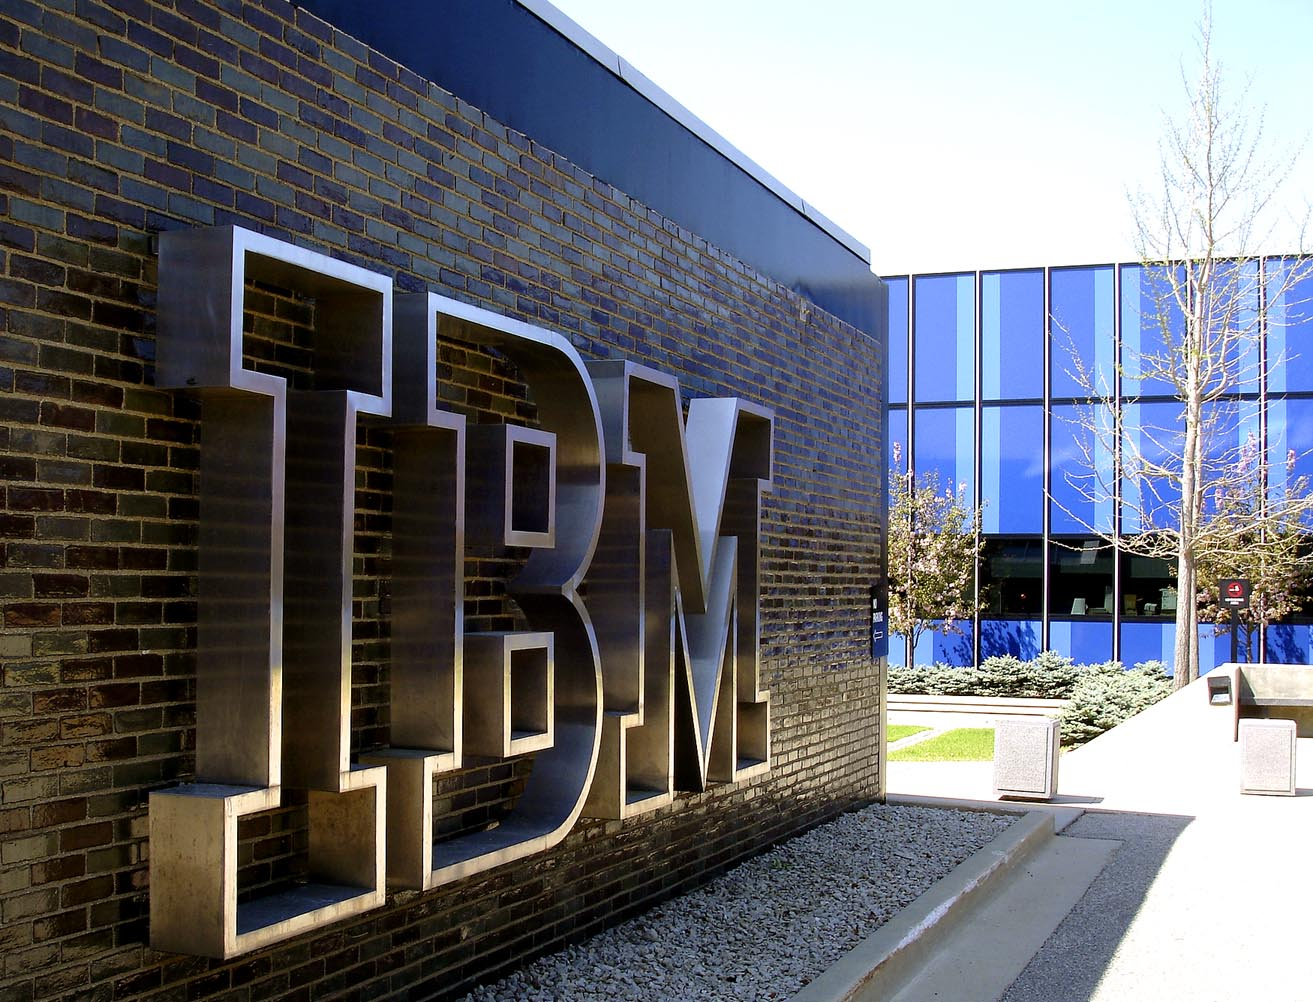
\includegraphics[width=5cm, height=3cm]{figuras/ibm.jpeg}
                \caption{IBM.}
                \label{f13} 
                \end{center}
            \end{figure}
            \item\textbf{Google} \par
            El gigante de la industria de la informática ofrece servicios a través de Google App Engine, que es una plataforma que ofrece construcción y alojamiento de aplicaciones web con la infraestructura de Google, donde solo se paga lo que se utiliza. \par Permite que los recursos informáticos  sean  fáciles  de  construir,  mantener  y  escalar  a  medida  que  crecen  las necesidades de almacenamiento y tráfico de web. \par La fijación de precios Google Cloud Storage se basa en una tarifa plana para su almacenamiento y una tasa de uso de la red.  \par El uso del almacenamiento de proyectos y uso de banda ancha se calculan en gigabytes (GB), permitiendo alcanzar hasta más de 90TB de uso.
            \begin{figure}[H]
                \begin{center}
                
\includegraphics[width=5cm, height=3cm]{figuras/google.jpeg}
                \caption{Google.}
                \label{f14} 
                \end{center}
            \end{figure}
        \end{enumerate}
    \end{itemize}
\end{enumerate}

\section{\textbf{Conclusiones}}
Este informe presentó información relevante acerca de los dispositivos de almacenamiento actuales, se ha explicado los conceptos teóricos relacionados con este, además de permitir conocer sobre la minería de datos y las tecnologías que almacenan grandes volúmenes de datos, que facilitan grabar e instalar nuestra información en softwares y tecnologías que se alejan enormemente de los almacenamientos que existía al principio, sino más bien a no poseer ningún dispositivo físicamente, solamente virtual. 
%-------------------------------------------------------
\medskip
\bibliography{refer}
\end{document}
